%% LyX 2.3.0rc2 created this file.  For more info, see http://www.lyx.org/.
%% Do not edit unless you really know what you are doing.
\documentclass[english]{scrartcl}
\usepackage[T1]{fontenc}
\usepackage[latin9]{inputenc}
\usepackage{color}
\usepackage{babel}
\usepackage{url}
\usepackage{pdfpages}
\usepackage{graphicx}
\usepackage[unicode=true,pdfusetitle,
 bookmarks=true,bookmarksnumbered=false,bookmarksopen=false,
 breaklinks=true,pdfborder={0 0 0},pdfborderstyle={},backref=false,colorlinks=true]
 {hyperref}

\makeatletter

%%%%%%%%%%%%%%%%%%%%%%%%%%%%%% LyX specific LaTeX commands.
%% Because html converters don't know tabularnewline
\providecommand{\tabularnewline}{\\}
%% A simple dot to overcome graphicx limitations
\newcommand{\lyxdot}{.}


\makeatother

\begin{document}

\titlehead{McIntire-Stennis Proposal}

\title{Guam Forest Biodiversity Inventory}

\author{Aubrey Moore}
\maketitle
\begin{center}
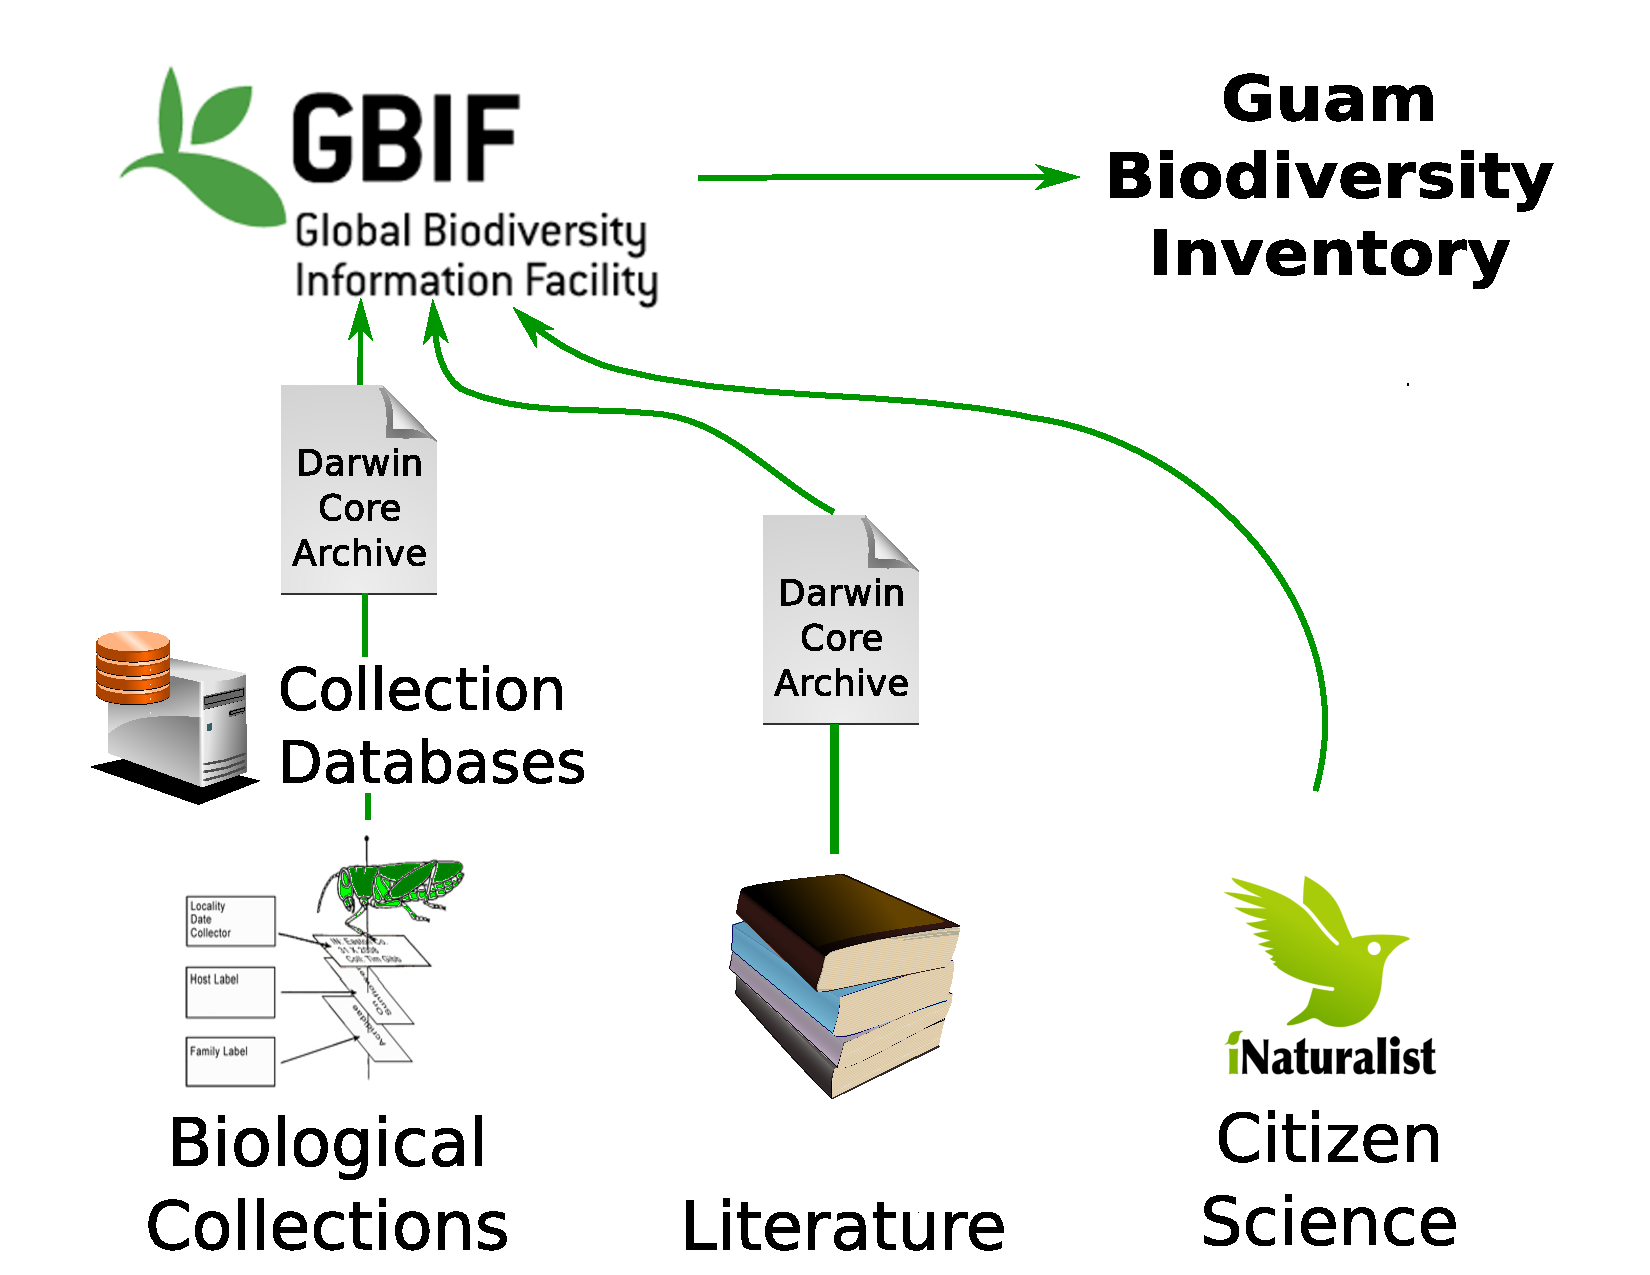
\includegraphics[scale=0.5]{diag1}
\par\end{center}

\newpage{}

\tableofcontents{}

\newpage{}

\section{Justification}

Funding is requested to support building and maintenance of a Guam
Forest Biodiversity Inventory. In its simplest form, a biodiversity
inventory is simple a checklist of taxa inhabiting a geographic area
or habitat of interest. In this case the habitat of interest is Guam's
forests. 

Guam's forest ecosystems are rapidly being degraded by invasive insect
species and habitat destruction. Impacts of bird extinctions caused
by brown treesnake predation on Guam's forests are well known. But
these impacts are rivaled by contemporary ecological disasters. Just
a couple of examples:
\begin{enumerate}
\item In 2002, a USDA Forest Service survey \cite{j.a.donnegonguamsforest}
reported that Guam's endemic cycad, \emph{Cycas micronesica}, was
the most abundant tree in Guam's forests. In 2003 the Asian cycad
scale, \emph{Aulacaspis yasumatsui}, was detected on Guam infesting
ornamental cycads. The scale quickly spread to wild cycads and started
killing them. Within only 3 years, \emph{Cycas micronesica} was placed
on the IUCN Red List of Threatened Species and in 2016, this plant
was placed on the US national endangered species list. It is estimated
that 90\% of Guam's cycads have been killed and there is no sign of
recovery.
\item The same Forest Service survey listed coconut palm, \emph{Cocos nucifera},
as Guam's second most abundant tree. Guam's palms are rapidly being
killed by coconut rhinoceros beetle, \emph{Oryctes rhinoceros}, first
detected on the island in 2007. It is likely that 50\% or more of
the island's coconut palms will be lost.
\end{enumerate}
Despite rapid destruction of Guam's forests, as illustrated by these
2 examples, we do not have even a basic checklist which can be used
to document changes in biodiversity.

We need a need a biodiversity inventory:
\begin{itemize}
\item to document changes to Guam's ecosystems
\item to document detection of and impacts caused by invasive species
\item to provide free, open access to information on Guam's flora and fauna
(including images and occurrence maps) to the global scientific community,
policy makers, and the public
\item to act as a repository for data from biological surveys and biological
collections
\item to provide links to scientific literature about taxa which occur on
Guam
\item to document ecological relationships among taxa such as hosts, predators,
parasites, and diseases
\end{itemize}
\newpage The Guam Forest Biodiversity Inventory will use the Global
Biodiversity Information Facility (GBIF) as a repository. A custom
web site will be built by the PI to serve as a public interface to
Guam biodiversity data stored on GBIF. Darwin Core Archives (DwCA)
will be used extensively for transferring data to and from GBIF.\label{lists}
\begin{itemize}
\item The Guam Biodiversity Inventory will facilitate automatic generation
and updates to lists such as: 
\item A list of all invasive species on Guam with year first recorded 
\item A list of new species described from specimens collected on Guam 
\item A list of observations for Guam\textquoteright s endangered species 
\item A list of Guam\textquoteright s native plants with associated herbivores
and pathogens 
\item A list of crops grown on Guam and pests and pathogens which attack
them 
\item A list of pests and associated biological control agents 
\item For any taxon, a literature reference list and links to images 
\item Taxonomic checklists and field guides with images
\end{itemize}

\section{Previous Work and Present Outlook }
\begin{itemize}
\item This proposal evolves from the PI's previous McIntire-Stennis project
entitled \emph{Guam Forest Insect Survey.}
\item The PI recently put the entire UOG insect collection catalog (34,808
specimen records) has recently been put online at \url{http://scan-bugs.org/portal/collections/misc/collprofiles.php?collid=180}
Digital images will be added.
\item The PI recently accessioned over 5,000 specimens of insect seed predators
from Benita Laird-Hopkins research, part of the Ecology of Bird Loss
Project.
\item The PI recently put 37,000 digital images of UOG herbarium sheets
online at \url{https://osf.io/qdg46/}. Next step is to link these
images with the herbarium database.
\item The PI designed Guam Biodiversity Inventory and made a presentation
on this at the recent Guam Island Sustainability Conference \cite{GuamBDIPresentation2018}.
\item The PI has contracted the Bishop Museum to make PDFs of primary entomological
literature for Guam, namely \emph{Insects of Guam I and Insects of
Guam II. }These\emph{ }volumes will be made available for public download
from the Bishop Museum web site. These books will be data mined for
forest biodiversity information.
\item The PI recently established an internship so that students can assist
in curating the UOG insect collection.
\end{itemize}

\section{Objectives }

\subsection{Liberate data from biological collections}

\subsubsection{Complete digitization of the UOG insect collection}

The UOG insect collection catalog has already been made available
online using Symbiota. Note that Symbiota uploads data to GBIF. Existing
images will be uploaded and linked to specimen data. Images will be
made for taxa which have not been previously imaged and these will
also be uploaded.

\subsubsection{Complete digitization of the UOG herbarium}

The existing herbarium catalog will be converted from a local database
to an online database using Symbiota or Specify. Both of these online
collection database managers upload to GBIF. 

\subsection{Liberate data from the Scientific Literature}

The PI will organize extraction of Guam biodiversity information from
primary scientific publications, starting with \emph{Insects of Guam
I }and \emph{II}.

\subsection{Build the Guam Forest Biodiversity Web Site}

The PI will launch a web site to serve as a portal to Guam forest
biodiversity data stored in GBIF.

Pages will be developed to dynamicly generate lists such as those
suggested above (\ref{lists}).

\subsection{Outreach / Citizen Science}

The PI will offer annual workshops on the use of iNaturalist, a cell
phone social networking app used by citizen scientists and naturalists
to record biodiversity observations with images and georeferencing.
iNaturalist data which is validated as \emph{research grade} by the
community is automatically uploaded to GBIF.

The PI will work with the UOG Center for Island Sustainability to
organize annual bioblitzes. A \href{https://en.wikipedia.org/wiki/BioBlitz}{bioblitz}
is is an intense period of biological surveying in an attempt to record
all the living species within a designated area.

\subsection{Collaboration}
\begin{itemize}
\item Collaboration with taxonomists will be cultivated to help identify
a large backlog of unidentified specimens in the UOG insect collection. 
\item Existing collaboration with existing partners list in section 7 will
be maintained.
\item The PI will participate in at least one scientific meeting cover biological
collections or biodiversity informatics per year. 
\item The PI will encourage donation of voucher specimens to the UOG insect
collection from biological surveys such as those being conducted by
the Ecology of Bird Loss and the baseline surveys being done by military
contractors in support of the military buildup.
\end{itemize}

\section{Duration and Timetable }

\subsection{Duration}

This performance period for this project will be 5 years. 

\subsection{Timetable}

\begin{tabular}{|l|c|c|c|c|c|}
\hline 
\textbf{Objective} & \textbf{Y1} & \textbf{Y2} & \textbf{Y3} & \textbf{Y4} & \textbf{Y5}\tabularnewline
\hline 
\hline 
1. Liberate data from Biological Collections & X &  &  &  & \tabularnewline
\hline 
2. Liberate data from the Scientific Literature &  & X & X & X & X\tabularnewline
\hline 
3. Build the Guam Forest Biodiversity Web Site & X & X &  &  & \tabularnewline
\hline 
4. Outreach / Citizen Science & X & X & X & X & X\tabularnewline
\hline 
5. Collaboration & X & X & X & X & X\tabularnewline
\hline 
\end{tabular}

\section{Financial Support/Budget}
\begin{description}
\item [{Staff~Salary}] \$8,000 per year will be used to fund an existing
student internship program. Interns assist in curation of the University
of Guam insect collection. Students will also assist in entering data
into the Guam Forest Biodiversity Inventory database.
\item [{Travel}] \$4,000 per year will facilitate UOG participation in
professional meetings and workshops on biological collections and
biodiversity informatics such as those hosted by the Integrated Digitized
Biocollections Project (iDigBio) and the Entomological Collections
Network (ECN). First year funding will allow the PI to attend the
ECN meeting associated with the Entomological Society of America meeting
in Vancouver during November 2018. Travel money may also be used to
support visits to Guam by taxonomists willing to identify specimens
in UOG collections.
\item [{Materials~and~Supplies}] \$4,000 per year will fund entomological
supplies required to maintain the UOG insect collection. Some of this
money will be used for shipping specimens for identification by taxonomists. 
\end{description}
\includepdf[pages=-]{\string"McStennis Budget Sheet template\string"}

\section{Personnel}
\begin{description}
\item [{Guam~Forest~Biodiversity~Inventory~Database}] The Guam Forest
Biodiversity Inventory database will be designed and maintained by
the PI with no direct cost to this project. Student interns will assist
with data entry.
\item [{University~of~Guam~Insect~Collection}] The University of Guam
Insect Collection is curated by the PI and Dr. Ross Miller with no
direct cost to this project. Student interns will assist with curation.
\item [{University~of~Guam~Herbarium}] The University of Guam Herbarium
is curated by Dr. Xiao Wei with database support from Dr. Tom Schills
with no direct cost to this project.
\end{description}

\section{Cooperation/Collaboration}
\begin{itemize}
\item Guam Plant Extinction Prevention Program (GPEPP)
\item Secretariat of the Pacific Regional Environment Program (SPREP)
\item International Union for the Conservation of Nature, Invasive Species
Specialist Group (IUCN ISSG)
\item University of Guam Herbarium
\item University of Guam Insect Collection
\item Guam Invasive Species Council (GISC)
\item Digitized Biocollections Project (IDigBio)
\item Entomological Collections Network (ECN)
\item Symbiota Collections of Arthropods Network (SCAN/Symbiota)
\item iNaturalist
\item University of Guam EPSCOR
\item University of Guam Center for Island Sustainability
\end{itemize}
\bibliographystyle{plainnat}
\bibliography{refs}

\end{document}
